\subsection{Other encodings}
\label{sec:data-other}

There are many other lossless data compression schemes described in the literature. Run-length encoding is one such method which encodes substrings consisting of repeated consecutive symbols, known as \textit{runs}, with their repeated symbol and length. First employed in 1967 for transmission of analogue television signals, run-length encoding proves beneficial when there are many runs, especially of long length \cite{rle}. Unfortunately, nanopore signal data does not contain many such runs and would likely encode poorly under this method.

Burrows-Wheeler transform is a data compression preprocessing step used to rearrange data in order to increase its number of runs \cite{bwt}. It is easily reversible, such that the original untransformed data can be obtained from the Burrows-Wheeler transformed data. It has been used to great effect in bioinformatics to compress to basecalled genomic data in the form of FASTQ files \cite{bwt-genomic}.

Stream VByte is a specialised codec for compressing 32-bit unsigned integers \cite{svb}. It stores each integer using a variable number of bytes (1 to 4) depending on its size. Integers in the range $[2^{8(n-1)},2^{8n}-1]$ are represented using $n>0$ bytes. For example, integers in the range $[1,255]$ are losslessly represented using 1 byte. The integer 0 is a special case missing from the above formula which is classically represented using 1 byte. There is however a variation which instead encodes 0 using 0 bytes and integers in the 3 byte range $[2^{16},2^{24}-1]$ with 4 bytes rather than 3. This is advantageous if 0 occurs more often than integers in the 3 byte range. See Tables \ref{tab:svb-classical} and \ref{tab:svb-0based} for a comparison of the classical and alternative encodings. The number of bytes used for each integer is stored in an array of control bytes which prefaces the actual data. 2-bit words are used to store the number of bytes used for each integer with 00, 01, 10 and 11 corresponding to 1, 2, 3 and 4 bytes respectively (or 0, 1, 2 and 4 bytes in the variation).

%\begin{tikzpicture}
 	%axis
	\draw (0,0) -- coordinate (x axis mid) (429.4967296,0);
    	\draw (0,0) -- coordinate (y axis mid) (0,4);
    	%ticks
    	\foreach \x in {0,0.0000256,0.0065536,1.6777216,429.4967296}
     		\draw (\x,1pt) -- (\x,-3pt)
			node[anchor=north] {\x};
    	\foreach \y in {0,...,4}
     		\draw (1pt,\y) -- (-3pt,\y)
     			node[anchor=east] {\y};
	%labels
	\node[below=0.8cm] at (x axis mid) {Unsigned 32-bit Integer};
	\node[rotate=90, above=0.8cm] at (y axis mid) {Bytes Used};

	%plots
	\draw (0,1) -- (0.0000256,1);
	\draw (0.0000256,2) -- (0.0065536,2);
	\draw (0.0065536,3) -- (1.6777216,3);
	\draw (1.6777216,4) -- (429.4967296,4);

\end{tikzpicture}

\begin{table}
    \caption{The number of bytes used and their control word encoding for different integer ranges in classical Stream VByte. \label{tab:svb-classical}}
    \begin{tabular}{|l|l|l|}%|p{4cm}|p{5.1cm}|}
        \hline
        Integer Range & Number of Bytes Used & Control Codeword\\
        \hline
	$[0,255]$ & 1 & 00\\
	$[256,65535]$ & 2 & 01\\
	$[65536,16777215]$ & 3 & 10\\
	$[16777216,4294967295]$ & 4 & 11\\
        \hline
    \end{tabular}
\end{table}

\begin{table}
    \caption{The number of bytes used and their control word encoding for different integer ranges in 0-based Stream VByte. \label{tab:svb-0based}}
    \begin{tabular}{|l|l|l|}%|p{4cm}|p{5.1cm}|}
        \hline
        Integer Range & Number of Bytes Used & Control Codeword\\
        \hline
	$\{0\}$ & 0 & 00\\
	$[1,255]$ & 1 & 01\\
	$[256,65535]$ & 2 & 10\\
	$[65536,4294967295]$ & 4 & 11\\
        \hline
    \end{tabular}
\end{table}

% put svb format figure here

Another variation to this encoding for 16-bit unsigned integers, known as Stream VByte 16, was developed by Oxford Nanopore Technologies in 2022 for compressing nanopore signal data in the POD5 file format \cite{pod5}. It is the same as the classical Stream VByte encoding described above except that each integer is stored using 1 or 2 bytes rather than 1 to 4 bytes. Since there are two different byte lengths, each of the byte lengths is stored using 1 bit; byte lengths 1 and 2 correspond to bit values 0 and 1 respectively. See Table \ref{tab:svb-16}. If each integer lies in the range $[0, 2^{16})$ this method saves one bit per integer on average versus classical Stream VByte. Due to their similarities, I hypothesise that the compression and decompression speed of Stream VByte 16 is similar if not better than classical Stream VByte. But there is no existing benchmark in the literature which compares both algorithms.

\begin{table}
    \caption{The number of bytes used and their control word encoding for different integer ranges in Stream VByte 16. \label{tab:svb-16}}
    \begin{tabular}{|l|l|l|}%|p{4cm}|p{5.1cm}|}
        \hline
        Integer Range & Number of Bytes Used & Control Codeword\\
        \hline
	$[0,255]$ & 1 & 0\\
	$[256,65535]$ & 2 & 1\\
        \hline
    \end{tabular}
\end{table}


This leads us to the current state-of-the-art approach for compressing nanopore signal data which we will name \textit{VBZ16}. VBZ16 is equivalent to VBZ \cite{vbz} but Stream VByte is replaced with Stream VByte 16. VBZ16 consists of the following encodings applied successively:

\begin{enumerate}
\item delta,
\item zig-zag,
\item Stream VByte 16 and
\item Zstandard \cite{zstd}.
\end{enumerate}

Delta encoding is a well-known technique

This requires at least four passes over the input data depending on how many passes Zstandard performs.
